\documentclass{report}

\usepackage{graphicx} % Required for inserting images
\usepackage{wrapfig}
\usepackage[table,xcdraw]{xcolor}
\usepackage{hyperref}
\usepackage[export]{adjustbox}
\usepackage{geometry}
\usepackage{listings}
\usepackage{caption}
\usepackage{subfigure}
\usepackage{tikz}
\usepackage{enumitem}
\usepackage{multirow}
\usepackage{forest}
\usepackage[bottom]{footmisc}
\usepackage{amsmath}
\usepackage{longtable}



\setcounter{secnumdepth}{3}
\setcounter{tocdepth}{3}
\geometry{a4paper,
 total={150mm,257mm},
 left=15mm,
 right=15mm,
 top=20mm}

 \begin{document}
  \tableofcontents

    
  \chapter{Crittografia Simmetrica}
  \section{Introduzione}
    Se parliamo di crittografia Simmetrica, stiamo considerando uno schema in cui sono presenti almeno 2 agenti (Bob, Alice) che devono scambiare un messaggio in maniera sicura senza che un terzo (che potrebbe avere intenzioni malevole) possa capire il messaggio. 
    Il modello quindi prevede una funzione di cifrazione (Enc) e una funzione di decifrazione (Dec), una chiave condivisa (k) e due tipi di messaggio, \textit{x} detto messaggio in chiaro (plaintext) e \textit{y} detto messaggio cifrato (ciphertext) ; la funzione di criptazione è determinata da un algoritmo che pubblicamente conosciuto, quello che invece rende sicuro l'utilizzo della cifratura simmetrica è la segretezza e lunghezza della chiave. 
    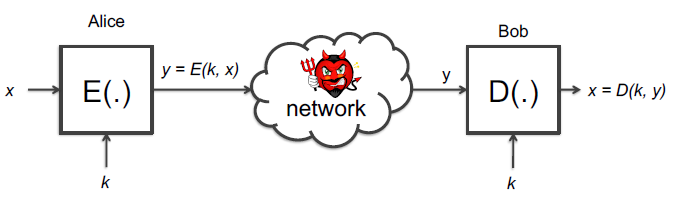
\includegraphics{./immagini/modello.png} 
    
    \subsubsection{Definizione di Cifrario}
        Un cifrario, o schema di cifratura, è defito su una tripletta composta da (K,P,C) usata nelle funzioni di (Gen,Enc,Dec) definite con questi domini: 
         \begin{align}
            &Gen: Z^+ \to K funzione generatrice di chiavi\\  
            &Enc: P \times K \to C  funzione di cifratura\\
            &Dec : C \times K \to P funzione di decifratura\\
            &x \in P , y \in C , k \in K\\
            &y = Enc(k,x)\\
            &x = Dec(k,y)
        \end{align}
        \paragraph{Proprieta di cifratura}
            La cifratura deve anche rispettare le seguenti proprieta: 
            \begin{description}
                 \item[Correttezza]: $\forall p \in P \land k \in K, \exists Dec(k,Enc(k,p)) = p$
                 \item[Sicurezza]:  Un cifrario simmetrico è sicuro $\iff \forall (p,c), p \in P \land c \in C  \Rightarrow$ 
                 \begin{itemize}
                            \item dato \textit{c} ciphertext, è "difficile" determinare \textit{p} plaintext senza conoscere la chiave \textit{k}, e viceversa
                            \item è "difficile" determinare \textit{k} chiave, ammenoche non sia stata già usata una volta
               \end{itemize}
            \end{description}

        \paragraph{Esempio : Sostituzione monoalfabetca} 
            Vediamo quindi un tipo di cifratura a sostituzione, dove la chiave è la permutazione dell' alfabeto. L' algoritmo prevede la sostituzione delle lettere della parola con le corrispondenti dell' alfabeto shiftato, e per decriptare si usa l' algoritmo al contrario. Le chiavi quindi possono essere circa  26! cioè circa $4\cdot10^26$, quindi tentare un attacco a forza bruta non è possibile, ma è possibile applicare tecniche di Crittoanalisi analizzando alcune proprietà che riguardano i linguaggi come : la frequenza delle lettere, la generalizzazione delle coppie e triple di lettere, la frequenza delle parole corte se sono identificati i separatori.  
    \subsubsection{Crittoanalisi}        
            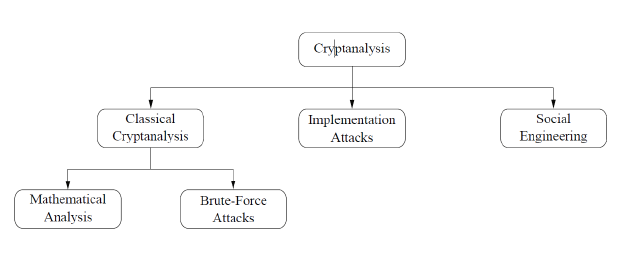
\includegraphics{./immagini/crittoanalisi.png}
               
          \paragraph{Complessità dell'attacco} Viene definito da:
                \begin{description}
                    \item[Complessità dei Dati:] Numero previsto di unità dei dati in ingresso richiesti.
                    \item[Complessità di Storage:] Numero previsto delle unità di storage richiesti.
                    \item[Complessità di Elaborazione:] Numero previsto di operazioni richiesti per processare i dati in input o/e per riempire la memoria con dati.
                \end{description}
            
           \paragraph{Tipi di attacco} Si possono classificare in:
               
                \begin{itemize}
                    \item Ciphertext-only attack
                    \item Known-plaintext attack
                    \item Chosen-plaintext attack (CPA)
                \end{itemize}
                Se un metodo è sicuro contro i CPA, allora è sicuro anche contro gli altri.
            \paragraph{Principi di Kerchoff}

            \begin{description}
                \item[Massima di Kerckhoffs] Un sistema crittografico dovrebbe rimanere sicuro anche se tutto del sistema, tranne la chiave, è di pubblico dominio.
                
                \item[Massima di Shannon] Il nemico conosce il sistema.
                
                \item[Massima di Bruce Schneier] Meno e più semplici sono i segreti da custodire per garantire la sicurezza del sistema, più facile sarà mantenerne la sicurezza.
            \end{description}

            \textbf{Consigli per mantenera la sicurezza facile}
            \begin{itemize}
                \item Le chiavi sono piccoli segreti.
                \item Conservare piccoli segreti è più facile che conservare grandi segreti.
                \item Sostituire piccoli segreti, una volta eventualmente compromessi, è più facile (ed economico) che sostituire grandi segreti.
            \end{itemize}

        \subsubsection{Esempi di cifrari} 
            \paragraph{Cifrario di cesare}

            Siano $PT$, $CT$ e $K$ elementi dell'anello $Z_{26}$.

            \begin{itemize}
                \item \textbf{Cifratura (Encryption):} \[
                y = x + k \mod 26
                \]
                
                \item \textbf{Decifratura (Decryption):} \[
                x = y - k \mod 26
                \]
                
                \item \textbf{Esempio:}
                \begin{itemize}
                    \item Testo in chiaro (Plaintext, $x$): ``\texttt{ATTACK}'' $\Rightarrow$ \[x = (0, 19, 19, 0, 2, 10)\]
                    \item Chiave ($k$): \[k = 17\]
                    \item Testo cifrato (Ciphertext, $y$): \[
                    y = (0+17, 19+17, 19+17, 0+17, 2+17, 10+17) \mod 26 = (17, 10, 10, 17, 19, 1)
                    \]
                    \item Risultato: ``\texttt{RKKRTB}''
                \end{itemize}
            \end{itemize}

            \paragraph{Cifrario Affine}

            \subparagraph{Definizione}

Siano $a, b, x, y \in Z_{26}$.

\begin{itemize}
    \item \textbf{Cifratura (Encryption):}
    \[
    y = a \cdot x + b \mod 26
    \]
    
    \item \textbf{Decifratura (Decryption):}
    \[
    x = a^{-1} \cdot (y - b) \mod 26
    \]
    
    \item La chiave è $k = (a, b)$, con $\gcd(a, 26) = 1$
    
    \item \textbf{Esempio:}
    \begin{itemize}
        \item Testo in chiaro (Plaintext): ``\texttt{ATTACK}'' $\Rightarrow (0, 19, 19, 0, 2, 10)$
        \item Chiave $k = (9, 13)$
        \item Cifratura:
        \[
        y = (9 \cdot x + 13) \mod 26
        \]
        \[
        y = (13, 2, 2, 13, 5, 25)
        \]
        \item Testo cifrato (Ciphertext): ``\texttt{NCCNFZ}''
    \end{itemize}
\end{itemize}

\subparagraph{Calcolo dello spazio delle chiavi}

Lo spazio delle chiavi si calcola come:
\[
\text{Spazio delle chiavi} = N_a \cdot N_b
\]

Dove:
\begin{itemize}
    \item $N_a$ è il numero di valori possibili di $a$ tali che $\gcd(a, 26) = 1$. \\
    In questo caso: $N_a = 12$
    \item $N_b$ è il numero dei possibili valori di shift $b$ in $Z_{26}$. \\
    Quindi: $N_b = 26$
\end{itemize}

Pertanto, lo spazio delle chiavi è:
\[
12 \cdot 26 = 312
\]


\section{Cifrario Perfetto}
  \subsection{Introduzione}
            Nel contesto della sicurezza crittografica, si considera un attaccante con la capacità di condurre un \textit{ciphertext-only attack}, ovvero un attacco in cui l'unica informazione disponibile è il testo cifrato.

            \paragraph{Requisiti di sicurezza}
                Un cifrario è considerato sicuro se soddisfa i seguenti requisiti:
            \begin{itemize}
                \item L'attaccante non è in grado di recuperare la chiave segreta.
                \item L'attaccante non è in grado di risalire al testo in chiaro (plaintext).
                \end{itemize}

            \paragraph{Intuizione di un cifrario perfettamente sicuro}
                L'idea alla base di un cifrario perfettamente sicuro è che, indipendentemente da qualsiasi informazione pregressa che l'attaccante possa avere sul testo in chiaro, il testo cifrato non deve fornire alcuna informazione aggiuntiva su di esso.
  \subsection{Approccio Probabilistico}
   Nel contesto della crittografia, il messaggio $M$ viene modellato come una variabile aleatoria, secondo una distribuzione di probabilità detta \textit{distribuzione del plaintext}. Ad esempio, si potrebbe avere:

  \begin{itemize}
      \item $\Pr[M = \text{``attack today''}] = 0.7$
      \item $\Pr[M = \text{``don't attack''}] = 0.3$
  \end{itemize}
  
  Queste probabilità rappresentano la \textit{conoscenza a priori} che un attaccante potrebbe avere riguardo al contenuto del messaggio.
  
  Il generatore di chiavi $\text{Gen}()$ definisce una distribuzione di probabilità sulla chiave $K$, ovvero:
  \[
  \Pr[K = k] = \Pr[k \leftarrow \text{Gen}()]
  \]
  Le variabili aleatorie $M$ (messaggio) e $K$ (chiave) si assumono indipendenti.
  
  \paragraph{Processo di generazione del ciphertext}
  \begin{enumerate}
      \item Si sceglie un messaggio $m$ secondo la distribuzione di $M$.
      \item Si genera una chiave $k$ da $\text{Gen}()$.
      \item Si calcola il testo cifrato $c \leftarrow E_k(m)$.
  \end{enumerate}
  
  Il testo cifrato $C$ risultante è anch'esso una variabile aleatoria, e il processo di cifratura definisce una distribuzione di probabilità indotta su $C$.

  \paragraph{Segretezza Perfetta}

  La \textit{segretezza perfetta} è un concetto fondamentale introdotto da Claude Shannon nel 1949. In modo informale, si riferisce alla condizione in cui il testo cifrato non rivela alcuna informazione sul testo in chiaro. Formalizziamo l'idea di ``informazione sul plaintext'' in termini di distribuzione di probabilità.
  
  Un sistema di cifratura gode di segretezza perfetta se, per ogni messaggio $m \in M$ e ogni testo cifrato $c \in C$ tale che $\Pr[C = c] > 0$, vale la seguente uguaglianza:
  \[
  \Pr[M = m \mid C = c] = \Pr[M = m]
  \]
  Questo implica che la probabilità a posteriori che un messaggio sia $m$, dato il testo cifrato $c$, è uguale alla probabilità a priori che il messaggio fosse $m$: osservare il testo cifrato non fornisce alcuna informazione aggiuntiva.
  
  Una formulazione equivalente della segretezza perfetta è la seguente:
  \[
  \forall m, m' \in M, \forall c \in C, \quad \Pr[E_k(m) = c] = \Pr[E_k(m') = c]
  \]
  In altre parole, la distribuzione del testo cifrato è indipendente dal messaggio originale. La distribuzione a priori del plaintext (prima di osservare il ciphertext) e quella a posteriori (dopo aver osservato il ciphertext) devono coincidere.
  
  \subsubsection{Teorema di Shannon}

  \paragraph{Teorema di Shannon}
  \begin{itemize}
      \item In un cifrario perfetto, $|K| \geq |M|$
      \item Ovvero, il numero di chiavi non può essere inferiore al numero di messaggi
  \end{itemize}
  
  \paragraph{Dimostrazione (per assurdo):}
  \begin{enumerate}
      \item Supponiamo che $|K| < |M|$
      \item Deve valere $|C| \geq |M|$, altrimenti il cifrario non è invertibile
      \item Quindi, $|C| > |K|$
      \item Sia $m \in M$ tale che $\Pr[M = m] \neq 0$; si calcoli $c_i \leftarrow E(k_i, m)$ per ogni $k_i \in K$
      \item Per il punto (3), esiste almeno un $c$ tale che $c \neq c_i$ per ogni $k_i \in K$
      \item Allora $\Pr[M = m \mid C = c] = 0$, che è diverso da $\Pr[M = m]$, contraddicendo la definizione di cifrario perfetto
  \end{enumerate}
  
  \paragraph{Fatto.} Sia $\Pi = (\text{Gen}, \text{Enc}, \text{Dec})$ uno schema di cifratura con $|M| = |K| = |C|$. Lo schema è perfettamente sicuro se e solo se:
  \begin{enumerate}
      \item  $\forall k \in K$ è scelto con probabilità uniforme $1/|K|$ da Gen
      \item  $\forall m \in M \land c \in C, \exists! k \in K : E_k(m) = c$
  \end{enumerate}
  
  \paragraph{Nota:}
  \begin{itemize}
      \item La condizione 1 è facile da verificare
      \item La condizione 2 non richiede il calcolo di probabilità
  \end{itemize}
  
  \subsubsection{Sicurezza incondizionata}
  La perfetta segretezza è equivalente alla sicurezza incondizionata. In questo modello, si assume che un avversario disponga di risorse computazionali illimitate. L'osservazione del testo cifrato non fornisce quindi alcuna informazione utile all'avversario riguardo al messaggio originale.
  
  \paragraph{Condizioni necessarie}
  \begin{itemize}
      \item I bit della chiave devono essere scelti in modo veramente casuale
      \item La lunghezza della chiave deve essere maggiore o uguale alla lunghezza del messaggio (secondo il teorema di Shannon)
  \end{itemize}
  
  \subsubsection{Indistinguibilità perfetta}
  Sia $\Pi = (G, E, D)$ uno schema di cifratura definito su insiemi $K$, $M$, $C$.
  
  $\Pi$ ha \emph{indistinguibilità perfetta} se e solo se:
  \[
  \forall m_1, m_2 \in M,\ |m_1| = |m_2|,\ \forall c \in C,\ \text{con } k \leftarrow G \text{ uniforme}:
  \quad \Pr[E(k, m_1) = c] = \Pr[E(k, m_2) = c]
  \]
  
  \subparagraph{Fatto}
  $\Pi$ ha indistinguibilità perfetta $\iff$ $\Pi$ è perfettamente sicuro.
  
            
    \subsection{One-Time Pad}
    Il \textit{One-Time Pad} è un sistema di cifratura brevettato da Vernam nel 1917, ma il suo principio era già noto circa 35 anni prima. È stato dimostrato perfettamente sicuro da Claude Shannon nel 1949. Un'applicazione celebre di questo metodo è il collegamento diretto e sicuro tra Mosca e Washington, noto come ``telefono rosso'', che in realtà non era un telefono ma un sistema di comunicazione sicura basato su teletype, fax e collegamenti informatici criptati.

    \subsubsection{Concetti preliminari}
    
    Il \textit{One-Time Pad} si basa sull'operazione logica \texttt{XOR} (OR esclusivo), definita dalla seguente regola:
    \[
    z = x \oplus y = (x + y) \mod 2
    \]
    
    \paragraph{Assunzioni}
    
    Sia $x \in \{0,1\}^t$ un messaggio binario di $t$ bit e $k \in \{0,1\}^t$ una chiave di pari lunghezza, i cui bit sono scelti in modo completamente casuale.
    
    \paragraph{Cifratura}
    
    Per ogni $i \in [1, \dots, t]$, il bit cifrato $y_i$ si ottiene come:
    \[
    y_i = m_i \oplus k_i \quad \text{ovvero} \quad y_i = (m_i + k_i) \mod 2
    \]
    
    \paragraph{Decifratura}
    
    Per ogni $i \in [1, \dots, t]$, si recupera il messaggio originale come:
    \[
    x_i = c_i \oplus k_i \quad \text{ovvero} \quad x_i = (y_i + k_i) \mod 2
    \]
    
    La proprietà di consistenza del sistema (cioè $x_i = m_i$ dopo cifratura e decifratura) è facilmente dimostrabile grazie alla simmetria dell'operazione \texttt{XOR}.
    
    \paragraph{XOR come buona funzione di cifratura}

\textbf{Teorema.} Sia $X$ una variabile aleatoria su $\{0,1\}^n$ e $K$ una variabile aleatoria indipendente e uniformemente distribuita su $\{0,1\}^n$. Allora $Y = X \oplus K$ è uniformemente distribuita su $\{0,1\}^n$.

\paragraph{Dimostrazione (caso $n = 1$)}
Siano $\Pr[X = 0] = X_0$ e $\Pr[X = 1] = X_1$, con $X_0 + X_1 = 1$.\\
Allora:
\[
\Pr[Y = 0] = \Pr[X = 0 \land K = 0] + \Pr[X = 1 \land K = 1] = X_0 \cdot 0.5 + X_1 \cdot 0.5 = 0.5 (X_0 + X_1) = 0.5
\]
e analogamente $\Pr[Y = 1] = 0.5$. Quindi $Y$ è uniforme.

\paragraph{Pro e contro dell'One-Time Pad}

L'One-Time Pad (OTP) è un sistema crittografico estremamente sicuro, ma presenta anche importanti limitazioni pratiche.

\subparagraph{Pro}
\begin{itemize}
    \item \textbf{Sicurezza incondizionata}: un sistema è detto incondizionatamente sicuro (o sicuro dal punto di vista dell'informazione) se non può essere violato nemmeno disponendo di risorse computazionali illimitate.
    \item \textbf{Ottimalità}: l'OTP è ottimale in quanto ogni chiave cifra un solo messaggio in un solo testo cifrato. Vale che $|M| = |K| = |C|$.
    \item \textbf{Efficienza}: la cifratura e decifratura sono operazioni estremamente veloci, basate su un semplice XOR bit a bit.
\end{itemize}

\subparagraph{Contro}
\begin{itemize}
    \item \textbf{Chiavi lunghe}: la chiave deve essere lunga quanto il messaggio, il che rende il sistema poco pratico. In generale, $|K| \geq |M|$.
    \item \textbf{Riutilizzo della chiave proibito}: la chiave deve essere usata una sola volta. Il riutilizzo (due-time pad) compromette la sicurezza. Se $C_1 = M_1 \oplus K$ e $C_2 = M_2 \oplus K$, allora $C_1 \oplus C_2 = M_1 \oplus M_2$.
    \item \textbf{Attacchi con testo in chiaro noto}: conoscendo una coppia $(m, c)$, si può ricavare direttamente la chiave $k = m \oplus c$.
    \item \textbf{Malleabilità}: il sistema è malleabile, cioè modifiche al testo cifrato si riflettono in modo prevedibile sul testo in chiaro senza essere rilevate.
\end{itemize}

\paragraph{Segretezza perfetta dell’One-Time Pad}

\textbf{Teorema.} Il cifrario One-Time Pad soddisfa la segretezza perfetta.

\paragraph{Dimostrazione}
\begin{enumerate}
    \item Per definizione di probabilità condizionata (legge di Bayes):
    \[
    \Pr[M = m \mid C = c] = \frac{\Pr[C = c \mid M = m] \cdot \Pr[M = m]}{\Pr[C = c]}
    \]
    \item Calcoliamo $\Pr[C = c]$ usando la legge della probabilità totale:
    \[
    \Pr[C = c] = \sum_i \Pr[C = c \mid M = m_i] \cdot \Pr[M = m_i] = \sum_i \Pr[K = c \oplus m_i] \cdot \Pr[M = m_i]
    \]
    Poiché $K$ è uniforme, $\Pr[K = c \oplus m_i] = 2^{-k}$:
    \[
    \Pr[C = c] = \sum_i 2^{-k} \cdot \Pr[M = m_i] = 2^{-k}
    \]
    \item Sostituendo nella formula iniziale:
    \[
    \Pr[M = m \mid C = c] = \frac{2^{-k} \cdot \Pr[M = m]}{2^{-k}} = \Pr[M = m]
    \]
\end{enumerate}

Quindi il testo cifrato non rivela alcuna informazione aggiuntiva sul messaggio: l'OTP ha segretezza perfetta.
\paragraph{Malleabilità}

Un sistema crittografico si dice \textit{malleabile} se un attaccante è in grado di trasformare un testo cifrato in un altro testo cifrato tale che il corrispondente testo in chiaro subisce una trasformazione prevedibile. In questo scenario, l’attaccante non decifra direttamente il messaggio, ma riesce comunque a manipolarlo in modo controllato e coerente, ottenendo un effetto noto sul contenuto in chiaro.

\paragraph{Sulla malleabilità dell'OTP}

Un esempio di attacco contro l'integrità di un sistema OTP si verifica quando un attaccante intercetta il testo cifrato e lo manipola in modo che il testo in chiaro risultante sia una versione trasformata ma prevedibile del messaggio originale.

\subparagraph{Attacco contro l'integrità}
\begin{itemize}
    \item Alice invia a Bob il testo cifrato $c = p \oplus k$, dove $p$ è il messaggio e $k$ è la chiave.
    \item L'avversario intercetta $c$ e trasmette a Bob un testo cifrato modificato $c' = c \oplus r$, dove $r$ è chiamato perturbazione.
    \item Bob riceve $c'$ e lo decifra: $p' = c' \oplus k = (c \oplus r) \oplus k = (p \oplus k) \oplus r \oplus k = p \oplus r$, ottenendo così $p' = p \oplus r$.
    \item La perturbazione $r$ passa inosservata e ha un impatto prevedibile sul testo in chiaro.
\end{itemize}



\textbf{RIGUARDARE GLI ESERCIZI SULLA PROBABILITÃ Slide 1.01}



\section{Stream Chipers}
    \subsubsection{Come faccio un OTP in pratica?}
    L'idea è usare, al posto di una chiave di stream completamente casuale, una chiave pseudo-casuale utilizzando uno \textit{Pseudo Random Generator} G che è una funzione efficiente e deterministica, che utilizza un \textit{seed} per generare poi un valore pseudo-casuale con 
    \[G: \{0,1\}^s(\text{Spazio del seed}) \rightarrow \{0,1\}^n (\text{spazio della Chiave}), n (\text{dimensioni della chiave}) \gg s (\text{dimensioni del seed})\]
    si ha quindi poi come funzione di criptazione $y = G(k) \oplus x$  e come funzione di decriptazione $x = G(k) \oplus y$ con \textit(k) che viene utilizzata come seed della funzione. 
    Si viene però a creare un problema ovvero il numero di chiavi $|k|$ è minore del numero di messaggi $|m|$, violando cosi il principio si Shannon. 
    La sicurezza dipenderà dallo specifico Generatore Pseudo-Casuale (PRG, in inglese Pseudo-Random Generator). È fondamentale che un PRG appaia casuale, ovvero che sia indistinguibile da un vero generatore casuale (TRG, True Random Generator) per un avversario con capacità limitate.

Deve essere computazionalmente irrealizzabile distinguere l'output di un PRG da quello di un TRG. Questo concetto introduce una nuova definizione di sicurezza: la \textbf{sicurezza computazionale}.

\paragraph{Sicurezza computazionale}
Un cifrario si dice \textbf{computazionalmente sicuro} (in modo pratico) se il livello percepito di computazione necessario per violarlo, utilizzando il miglior attacco noto, supera, con un buon margine, le risorse computazionali dell’avversario ipotizzato.

In questa prospettiva, l'avversario viene considerato come avente una potenza di calcolo limitata. Tuttavia, è fondamentale porsi la domanda: qual è il miglior attacco conosciuto? Anche se si conosce un limite inferiore della complessità di un attacco, non si può escludere che esistano attacchi più potenti e non ancora scoperti.

Pertanto, la miglior strategia attuale è progettare sistemi crittografici assumendo che siano \textbf{computazionalmente sicuri}.

\paragraph{Imprevedibilità del PRG}
Un PRG, oltre ad avere buone proprietà statistiche, deve essere \textbf{imprevedibile}. Se un PRG risulta prevedibile, allora un cifrario a flusso che lo utilizza non può essere considerato sicuro.

Supponiamo che un avversario sia in grado di determinare un prefisso della sequenza generata \( x \). In tal caso, egli può calcolare un prefisso del keystream (flusso di chiavi). Se la funzione di generazione \( G \) è prevedibile, l’avversario potrà calcolare anche il resto del keystream, riuscendo quindi a decifrare il messaggio cifrato \( y \).

\paragraph{Imprevedibilità in avanti}
L’\textbf{imprevedibilità in avanti} richiede che, se il seme iniziale (seed) non è noto, allora il prossimo bit della sequenza generata deve essere imprevedibile, indipendentemente dalla conoscenza di un qualsiasi prefisso della sequenza.

\paragraph{Imprevedibilità all’indietro}
L’\textbf{imprevedibilità all’indietro} implica che non deve essere possibile risalire al seme a partire dalla conoscenza di una qualsiasi porzione della sequenza generata.

In sintesi, anche se una sequenza appare o si comporta come casuale, non deve essere possibile prevedere né i bit successivi né risalire al seme che ha generato la sequenza.
 
\begin{figure}[h]
    \centering
    \includegraphics{./immagini/TRBG.png}
    \caption{Schema di generazione di una sequenza pseudocasuale. 
    Un processo casuale vero (true random process) genera una sequenza casuale attraverso una fase di digitalizzazione. 
    Questa sequenza casuale può essere utilizzata come \textit{seed} per un generatore pseudocasuale (PRBG, \textit{Pseudorandom Bit Generator}),
    il quale produce una sequenza pseudocasuale. Il contesto applicativo può influenzare il comportamento del PRBG.}
\end{figure}

\subsection{State of Art e Casi studio}
    \subsubsection{WEP}
    Nel protocollo 802.11b WEP, viene utilizzata una chiave segreta $k$ di lunghezza fissa pari a 104 bit. Per ogni nuovo messaggio viene scelto un nuovo IV (Initialization Vector), lungo 24 bit. L'uso dell'IV serve ad evitare l'utilizzo dello stesso keystream per due messaggi diversi, condizione nota come two-time pad (2TP), che comprometterebbe la sicurezza.

La procedura di cifratura prevede che il messaggio $m$ venga concatenato al suo checksum (calcolato tramite una funzione CRC), e poi cifrato utilizzando un keystream generato da una funzione pseudocasuale, la quale prende come input la concatenazione dell'IV e della chiave $k$, ovvero $PRG(IV || k)$. Il pacchetto trasmesso contiene l'IV in chiaro seguito dal ciphertext.

Tuttavia, la limitata lunghezza dell'IV (24 bit) implica che, dopo circa $2^{24} \approx 16$ milioni di frame trasmessi, è probabile che si verifichino ripetizioni dell'IV. Inoltre, su alcune schede 802.11, l'IV viene semplicemente incrementato frame dopo frame (ad esempio, chiave per il frame \#1: $1||k$, per il frame \#2: $2||k$, per il frame \#3: $3||k$, e così via), e in alcuni casi, dopo un ciclo di spegnimento e riaccensione, l'IV viene azzerato. Queste pratiche generano chiavi strettamente correlate tra loro, anziché casuali, riducendo drasticamente la sicurezza del sistema.

A causa di queste debolezze, nel 2001 Fluhrer, Mantin e Shamir (FMS) hanno dimostrato che è possibile recuperare la chiave $k$ osservando circa $10^6$ frame cifrati. Con miglioramenti successivi all'attacco, oggi bastano circa 40.000 frame per compromettere la chiave. È quindi fondamentale evitare la generazione di chiavi correlate e preferire costruzioni più sicure, dove ogni frame dispone di una chiave pseudocasuale indipendente.


\subsubsection{Linear Feedback Shift Register (LFSR)}
Il Linear Feedback Shift Register (LFSR) è un circuito digitale utilizzato per generare sequenze di bit pseudo-casuali. È composto da un registro a scorrimento, costituito da celle di memoria (flip-flop), e da una logica di retroazione che combina i valori presenti nelle celle attraverso operazioni di somma modulo 2 (XOR).
\includegraphics{./immagini/LFSR.png}
\subparagraph{Funzionamento}
Ad ogni impulso di clock, il contenuto delle celle viene fatto scorrere verso destra e il nuovo bit da inserire nella cella più a sinistra viene calcolato come combinazione lineare dei bit precedenti, in base a specifici coefficienti di retroazione $p_j$. Se un coefficiente $p_j$ è pari a 1, significa che il bit corrispondente partecipa al calcolo della retroazione; se è 0, non partecipa. Formalmente, il nuovo bit generato $s_{i+m}$ è calcolato come:
\[
s_{i+m} = \sum_{j=0}^{m-1} p_j \cdot s_{i+j} \mod 2
\]
dove $m$ è il grado del registro, ovvero il numero di celle di memoria.

\paragraph{Proprietà degli LFSR}
\subparagraph{Seed}
Il \emph{seed} è lo stato iniziale del registro. È fondamentale che il seed non sia tutto composto da zeri, poiché in tal caso l'LFSR rimarrebbe bloccato permanentemente nello stato nullo, senza generare alcuna sequenza utile.

\subparagraph{Grado}
Il grado dell'LFSR è definito come il numero di celle di memoria presenti nel registro. Ad esempio, se sono presenti 8 flip-flop, si dice che l'LFSR ha grado 8.

\subparagraph{Periodicità}
La sequenza di bit generata da un LFSR è \emph{periodica}. Questo significa che, dopo un certo numero di cicli, la sequenza di stati del registro si ripete identicamente.

\subparagraph{Massima lunghezza}
Un LFSR può generare una sequenza di lunghezza massima pari a $2^m - 1$, dove $m$ è il grado del registro. Questa proprietà è garantita solo se i coefficienti di retroazione sono scelti opportunamente. In particolare, esiste un teorema che afferma che la lunghezza massima della sequenza generata da un LFSR di grado $m$ è $2^m - 1$. Gli LFSR che raggiungono questa lunghezza massima sono detti \emph{maximum-length LFSR} e possono essere facilmente costruiti con una scelta adeguata dei tap di retroazione.

\paragraph{Pro e contro degli LFSR}
Gli LFSR presentano numerosi vantaggi, ma anche alcune debolezze significative che è importante considerare attentamente.

\subparagraph{Vantaggi}
Uno dei principali punti di forza degli LFSR è che producono sequenze di bit con ottime proprietà statistiche. Le sequenze generate sono bilanciate (hanno circa lo stesso numero di 0 e di 1) e hanno buone proprietà di autocorrelazione, il che li rende ideali per applicazioni in ambito di crittografia e comunicazioni digitali, come la generazione di chiavi o il riempimento di canali.

\subparagraph{Svantaggi}
Nonostante le buone proprietà statistiche, gli LFSR sono strutture \emph{periodiche}, cioè la sequenza generata si ripete dopo un numero finito di passi. Inoltre, sono dispositivi \emph{lineari}, e questa linearità li rende vulnerabili ad attacchi crittografici sofisticati.

\paragraph{Attacco Known-Plaintext contro LFSR}
Gli LFSR sono particolarmente vulnerabili a un tipo di attacco chiamato \emph{Known-Plaintext Attack}. Questo attacco si articola in tre fasi principali:
\begin{enumerate}
    \item L'avversario raccoglie almeno $2m$ coppie di testo in chiaro ($pt$) e testo cifrato ($ct$), dove $m$ è il grado dell'LFSR.
    \item Utilizzando queste coppie, l'avversario è in grado di determinare un prefisso della sequenza $s_i$ generata dall'LFSR.
    \item Infine, l'avversario risolve un sistema di $m$ equazioni lineari in $m$ incognite per determinare i coefficienti di retroazione $p_j$. Una volta ottenuti questi coefficienti, può ricostruire completamente l'LFSR e prevedere tutta la sequenza futura.
\end{enumerate}

\paragraph{Gli LFSR devono essere abbandonati?}
Nonostante le vulnerabilità individuate, gli LFSR non devono essere necessariamente scartati. Una soluzione consiste nell'utilizzare una combinazione \emph{non lineare} di più LFSR per costruire cifrari robusti. Un esempio tipico è quello di utilizzare operazioni logiche come l'AND tra i segnali di uscita di diversi LFSR, aumentando così la complessità e la sicurezza del sistema risultante. Un esempio concreto di questo approccio è il cifrario Trivium, progettato nel 2003, che combina più registri a scorrimento tramite operazioni non lineari per ottenere una robustezza crittografica elevata.

\paragraph{State of the Art}
Nel panorama attuale della cifratura a flusso, esistono differenti approcci, principalmente suddivisi tra soluzioni orientate al software e soluzioni orientate all'hardware.

\subparagraph{Software Oriented}
Tra i cifrari a flusso orientati al software si annoverano algoritmi come RC4 e SEAL. Entrambi sono stati ampiamente studiati e analizzati dalla comunità scientifica, risultando generalmente sicuri, anche se l'uso di RC4 oggi è sconsigliato in nuovi progetti a causa di alcune vulnerabilità emerse nel tempo.

\subparagraph{Hardware Oriented}
Per quanto riguarda le implementazioni hardware, molte soluzioni si basano su registri a scorrimento con retroazione lineare (LFSR). Tuttavia, molte di queste soluzioni sono state compromesse nel tempo. Un esempio emblematico è dato dagli algoritmi di cifratura GSM, A5/1 e A5/2. A5/1 era originariamente un algoritmo segreto, ma è stato successivamente decifrato attraverso operazioni di reverse engineering. A5/2, invece, presenta vulnerabilità ancora più gravi e può essere attaccato in tempi relativamente brevi. Attualmente, né A5/1 né A5/2 sono raccomandati per garantire comunicazioni sicure. A5/3, noto anche come KASUMI, rappresenta un miglioramento significativo: è infatti un cifrario a blocchi, e non più un puro cifrario a flusso.

\subparagraph{eSTREAM Project}
Per migliorare la situazione dei cifrari a flusso, è stato lanciato il progetto eSTREAM, parte della ECRYPT Network of Excellence. L'obiettivo era selezionare cifrari moderni e sicuri adatti a diverse applicazioni. Il progetto ha raccolto 34 candidati, suddivisi in due profili:
\begin{itemize}
    \item \textbf{Profilo 1}: Cifrari a flusso destinati ad applicazioni software con requisiti di alta velocità di trasmissione. Tra i principali candidati troviamo HC-128, Rabbit, Salsa20/12 e SOSEMANUK.
    \item \textbf{Profilo 2}: Cifrari a flusso progettati per applicazioni hardware con risorse limitate. In questo contesto si distinguono Grain v1, MICKEY v2 e Trivium.
\end{itemize}

\subparagraph{Performance dei cifrari eSTREAM}
I risultati ottenuti nel progetto eSTREAM hanno mostrato performance molto promettenti. Su una piattaforma AMD Opteron da 2.2 GHz con sistema operativo Linux, sono state misurate le seguenti velocità:
\begin{itemize}
    \item RC4: 126 Mb/s
    \item Salsa20/12: 643 Mb/s
    \item SOSEMANUK: 727 Mb/s
\end{itemize}
Questi risultati evidenziano come i cifrari di nuova generazione riescano a superare di gran lunga le prestazioni di RC4, offrendo allo stesso tempo una maggiore sicurezza.

\subsection{CONTENT SCRAMBLING SYSTEM (CSS)}

Il Content Scrambling System (CSS) è un sistema di cifratura utilizzato per proteggere i contenuti, ad esempio nei DVD. Alla base del sistema ci sono due LFSR (Linear Feedback Shift Registers) il cui stato iniziale è determinato da un \emph{seed} o chiave di 5 byte, pari a 80 bit.

\paragraph{Funzionamento di ogni round}
Durante ogni round di generazione del flusso di chiavi, si eseguono 8 cicli di clock. In ogni ciclo, ciascun LFSR produce 8 bit di output. Gli output dei due LFSR vengono poi sommati modulo 256 per ottenere un byte di keystream. Per semplicità, il bit di riporto generato dall'addizione viene trascurato.

\paragraph{Vulnerabilità}
Il CSS risulta estremamente vulnerabile: può essere rotto con una complessità di appena $2^{17}$ operazioni, un valore molto inferiore rispetto alla complessità attesa di $2^{40}$.

\paragraph{Attacco Known Plaintext}
L'attacco sfrutta il fatto che un prefisso del filmato, pari a circa 20 byte, è noto in chiaro (ad esempio, i primi 20 byte di un file MPEG). Questo consente di ricavare direttamente un prefisso corrispondente del keystream. Conoscendo questa parte iniziale del keystream, diventa possibile ricostruire il seed iniziale.

\paragraph{Algoritmo di attacco}
L'attacco procede come segue:
\begin{enumerate}
    \item Si considerano tutte le possibili configurazioni iniziali di LFSR17, pari a $2^{17}$ possibilità.
    \item Per ogni configurazione, si esegue LFSR17 per ottenere i primi 20 byte di output.
    \item Si sottrae questo output dal prefisso noto del keystream per ottenere un candidato output di LFSR25.
    \item Si verifica se il candidato è coerente con il funzionamento di LFSR25:
    \begin{itemize}
        \item Se è coerente, si è trovato il corretto stato iniziale di entrambi gli LFSR e l'algoritmo termina.
        \item Altrimenti, si passa alla configurazione successiva di LFSR17 e si ripete il processo.
    \end{itemize}
\end{enumerate}
Una volta individuato il seed corretto, è possibile generare l'intero output del CSS. La complessità massima dell'attacco è quella di testare tutte le possibili configurazioni iniziali di LFSR17, ovvero $2^{17}$ tentativi.


\subsection{RBG}
\subsubsection{Definizione}

Un \textbf{Random Bit Generator} (RBG) è un generatore che produce una sequenza di bit statisticamente indipendenti e non polarizzati.

\paragraph{Indipendenza statistica}
L'indipendenza statistica implica che la probabilità di emissione di un valore di bit (0 oppure 1) non dipende dai bit precedentemente generati. In altre parole, ogni bit è generato senza alcuna influenza dai bit passati.

\paragraph{Assenza di polarizzazione}
L'assenza di polarizzazione (unbiased) significa che la probabilità di generare un bit 0 oppure 1 è esattamente pari a \( 0.5 \). Ogni bit ha quindi la stessa probabilità di assumere uno dei due valori possibili.

\paragraph{Random Number Generator (RNG)}
I \textbf{Random Number Generator} (RNG) possono essere utilizzati per generare numeri casuali distribuiti uniformemente. Un numero casuale nell’intervallo \([0, n]\) può essere ottenuto generando una sequenza casuale di bit di lunghezza \( \lceil \log_2(n+1) \rceil \) e convertendola in un intero.

Se il numero risultante supera \( n \), una possibile soluzione consiste nello scartarlo e nel generare una nuova sequenza casuale di bit, ripetendo il processo fino a ottenere un numero valido.

\paragraph{Classi di RBG}
Esistono diverse classi di Random Bit Generator:
\begin{itemize}
    \item \textbf{True Random Bit Generator (TRBG)}: generatori di bit veramente casuali, basati su fenomeni fisici imprevedibili.
    \item \textbf{Pseudorandom Bit Generator (PRBG)}: generatori di bit pseudocasuali, che producono sequenze apparentemente casuali ma deterministiche a partire da un seme iniziale.
    \item \textbf{Cryptographically Secure Pseudorandom Bit Generator (CSPRBG)}: una particolare categoria di PRBG progettata per soddisfare criteri di sicurezza crittografica, rendendo impraticabile per un avversario prevedere parti della sequenza o risalire al seme.
\end{itemize}


\subsubsection{True Random Bit Generators (TRBG) Hardware-based}

I \textbf{True Random Bit Generators} (TRBG) hardware-based si basano su fenomeni fisici che sono naturalmente casuali. Questi generatori sfruttano eventi o processi fisici imprevedibili per produrre sequenze di bit che non possono essere riprodotte in modo deterministico.

\paragraph{Fenomeni fisici utilizzati}
Ecco alcuni esempi di fenomeni fisici che possono essere utilizzati per generare casualità:
\begin{itemize}
    \item \textbf{Tempo trascorso tra l'emissione di particelle durante il decadimento radioattivo}: Il decadimento radioattivo è un processo fondamentale per la generazione di numeri casuali, in quanto è intrinsecamente casuale e non può essere previsto.
    \item \textbf{Rumore termico da un diodo semiconduttore o da una resistenza}: Il rumore termico è una fluttuazione casuale che si verifica a livello microscopico nei semiconduttori e che può essere misurato per generare numeri casuali.
    \item \textbf{Instabilità di frequenza di un oscillatore a libera corsa}: Gli oscillatori, come quelli in un circuito elettronico, possono mostrare instabilità di frequenza che sono casuali nel tempo.
    \item \textbf{Carica di una capacità metal-insulator-semiconductor durante un periodo di tempo fisso}: La carica su un condensatore può essere utilizzata per generare valori casuali, in base alla fluttuazione della carica accumulata nel tempo.
    \item \textbf{Turbulenza dell'aria all'interno di un disco rigido sigillato}: La turbolenza dell'aria che causa fluttuazioni casuali nei tempi di latenza durante la lettura dei settori di un disco rigido può essere un'altra fonte di casualità.
    \item \textbf{Suono da un microfono o video da una fotocamera}: Anche i suoni o i segnali video provenienti da fonti fisiche come microfoni o telecamere possono essere utilizzati per generare bit casuali.
\end{itemize}

\paragraph{Esempio: Intel Digital Random Number Generator}
Un esempio di TRBG hardware-based è il \textbf{Intel Digital Random Number Generator} (DRNG), introdotto nelle CPU Intel a partire dal 2012. Questo generatore si basa sullo standard NIST SP 800-90 e sfrutta le fluttuazioni del rumore termico all'interno della CPU per produrre numeri casuali. Il DRNG è controllato tramite le istruzioni \texttt{RDRAND} e \texttt{RDSEED} in linguaggio assembly, e sebbene sia parzialmente documentato, rimane una soluzione potente per la generazione di numeri casuali a livello hardware.

\paragraph{Limitazioni e malfunzionamenti}
Tuttavia, i TRBG hardware-based non sono esenti da problemi:
\begin{itemize}
    \item \textbf{Suscettibilità a influenze esterne}: I generatori di numeri casuali hardware-based possono essere soggetti a osservazione e manipolazione esterna, che potrebbero compromettere la qualità dell'output.
    \item \textbf{Test periodici}: È necessario effettuare test periodici per garantire che i generatori funzionino correttamente.
    \item \textbf{Guasti nei generatori}: I guasti possono manifestarsi sotto forma di generatori che producono sequenze di bit \textbf{polarizzate} o \textbf{correlate}, compromettendo la qualità dei numeri casuali generati.
    \item \textbf{Generazione di sequenze polarizzate}: Quando la probabilità di generare un 1 non è uguale alla probabilità di generare uno 0 (ad esempio, \( \Pr[1] \neq 0.5 \)), si ha una sequenza polarizzata.
    \item \textbf{Generazione di sequenze correlate}: Quando la probabilità di generare un 1 dipende dal bit precedente, si ha una correlazione tra i bit generati.
\end{itemize}

\paragraph{Tecniche di "deskewing"}
Per correggere i guasti nei generatori di numeri casuali hardware-based, vengono adottate tecniche di \textbf{deskewing}, che mirano a rimuovere eventuali bias (polarizzazioni) nei bit generati. Una tecnica pratica consiste nel passare la sequenza di bit attraverso una funzione di hash crittograficamente sicura per garantire che l'output finale sia casuale e privo di bias.

\paragraph{Esempio di deskewing}
Supponiamo che un generatore produca bit polarizzati ma non correlati, e che la probabilità di generare un 1 sia \( p \), con \( 0 < p < 1 \). Per rimuovere il bias nei bit, possiamo procedere nel seguente modo:
\begin{itemize}
    \item Raggruppare la sequenza di output in coppie di bit.
    \item Trasformare la coppia \texttt{10} in un 1, la coppia \texttt{01} in un 0, e scartare le coppie \texttt{00} e \texttt{11}.
    \item La sequenza risultante sarà sia priva di bias che non correlata.
\end{itemize}

\subsubsection{True Random Bit Generators (TRBG) Software-based}

I generatori di bit casuali basati su software, sebbene possano sembrare meno robusti rispetto a quelli hardware-based, sono comunque soggetti a osservazione e manipolazione. Tuttavia, possono essere migliorati utilizzando diverse fonti di casualità per creare numeri casuali di alta qualità.

\paragraph{Uso di fonti multiple di casualità}
Per migliorare la qualità dei numeri casuali, i generatori software-based dovrebbero sfruttare il maggior numero possibile di fonti di casualità. Queste fonti includono:
\begin{itemize}
    \item \textbf{Funzioni di mescolamento (mixing functions)}: Funzioni crittografiche sicure come gli hash (ad esempio SHA-1, MD5) possono essere utilizzate per mescolare i dati provenienti da diverse fonti.
    \item \textbf{Clock di sistema}: Il tempo di sistema (ad esempio, la data e l'ora correnti) è una fonte di casualità, sebbene possa essere prevedibile se non ben protetto.
    \item \textbf{Tempo trascorso tra battiture di tasti o movimento del mouse}: Le variazioni nel comportamento dell'utente possono fornire una buona fonte di casualità.
    \item \textbf{Contenuto dei buffer di input/output}: I dati che vengono scritti o letti da vari buffer di sistema possono essere utilizzati per generare numeri casuali.
    \item \textbf{Input dell'utente}: Eventi come le scelte o le interazioni dell'utente possono essere una fonte di casualità.
    \item \textbf{Valori del sistema operativo}: Ad esempio, il carico di sistema, le statistiche di rete o altre metriche operative possono fornire dati casuali aggiuntivi.
\end{itemize}

paragraph{Esempio: RNG basato su software – il caso di Linux}
Il kernel Linux implementa un RNG software-based che aggrega molteplici sorgenti di entropia, dette \texttt{src\_i}, dove ogni \texttt{i}-esima sorgente può essere, per esempio, il tempo tra due pressioni di tasti o tra due interruzioni hardware. I bit effettivi vengono poi estratti da due dispositivi a caratteri distinti:
\begin{itemize}
    \item \texttt{/dev/random}: fornisce numeri di qualità più elevata, ma blocca (blocking) la lettura finché non è disponibile sufficiente entropia.
    \item \texttt{/dev/urandom}: fornisce numeri ininterrottamente (non blocking), anche se con un livello di sicurezza leggermente inferiore in assenza di nuova entropia.
\end{itemize}
All’avvio del sistema, la cosiddetta \emph{boot time randomness} viene raccolta rapidamente per inizializzare lo stato interno del generatore, garantendo fin da subito una base di entropia accettabile senza attendere il naturale accumulo di eventi.```

\subsubsection{Pseudo Random Bit Generator (PRBG)}

\paragraph{Definizione}
Un \textbf{Pseudo Random Bit Generator} (PRBG) è un algoritmo deterministico che, dato un sequenza binaria veramente casuale di lunghezza \(k\) (seme), produce una sequenza binaria di lunghezza \(L\) (sequenza di bit pseudocasuali), dove \(L \gg k\).

Il numero massimo di sequenze possibili che il PRBG può generare è \(2^k\), cioè una frazione \( \frac{2^k}{2^L} \) di tutte le possibili sequenze.

\paragraph{Intuizione di Sicurezza}
Un seme “piccolo” viene espanso in una sequenza “grande” di bit pseudocasuali in modo tale che un avversario non possa distinguere “efficientemente” tra gli output di un PRBG e gli output di un True Random Generator (TRG).

\paragraph{Requisito di Sicurezza Minimo}
La lunghezza \(k\) del seme deve essere sufficientemente grande affinché sia “infeasible” (non praticabile) effettuare una ricerca tra \(2^k\) possibili sequenze di output, il che è una condizione necessaria per garantire la sicurezza del generatore.

\paragraph{Formalizzazione}
Per tutti gli attaccanti (test) \(A\), esiste una funzione trascurabile \( \epsilon(n) \), tale che:
\[
\Pr_{x \gets U_k}[A(G(x)) = 1] - \Pr_{y \gets U_{\ell(k)}}[A(y) = 1] \leq \epsilon(n)
\]
dove \(G\) è una funzione che mappa \(\{0, 1\}^k \rightarrow \{0, 1\}^\ell(k)\), \(x\) è campionato uniformemente da \(\{0, 1\}^k\), e \(U_k\) è la distribuzione uniforme su stringhe di \(k\) bit, mentre \(U_\ell(k)\) è la distribuzione uniforme su stringhe di \(\ell(k)\) bit.

\paragraph{Tipicamente}
Il generatore PRBG utilizza una sequenza ricorsiva, in cui il seme \(s_0\) è il seme iniziale e la sequenza viene generata iterativamente come segue:
\[
s_{i+1} = f(s_i), \quad i = 0, 1, 2, \dots
\]
dove \(f\) è una funzione deterministica che applica una trasformazione sullo stato precedente per produrre il prossimo stato.

\paragraph{Generalizzazione}
In un caso più generale, il PRBG può evolversi secondo una relazione che dipende non solo dallo stato precedente \(s_i\), ma anche da stati precedenti multipli \(s_i, s_{i-1}, s_{i-2}, \dots, s_{i-t}\). In questo caso, la relazione evolutiva potrebbe essere:
\[
s_{i+1} = f(s_i, s_{i-1}, s_{i-2}, \dots, s_{i-t})
\]
Questa generalizzazione permette al PRBG di avere un comportamento più complesso e una maggiore capacità di produrre sequenze più difficili da prevedere.
\paragraph{Linear Congruential Generator}
Il \emph{Linear Congruential Generator} (LCG) è uno dei generatori pseudocasuali più semplici e diffusi, spesso impiegato per scopi di simulazione e testing. La sua definizione formale è la seguente:
\[
\begin{aligned}
s_0 &= \text{seed},\\
s_{i+1} &= (a \cdot s_i + b)\bmod m,\quad i = 0,1,2,\dots,
\end{aligned}
\]
dove \(a\), \(b\) e \(m\) sono costanti intere opportunamente scelte.

Un esempio noto è la funzione \texttt{rand()} in ANSI C:
\begin{verbatim}
    s[0] = 12345;
    s[i] = (1103515245 \cdot s[i-1] + 12345) mod 2^{31};
\end{verbatim}

Supponiamo di conoscere un prefisso \(s_r, s_{r+1}, s_{r+2}\). Possiamo allora scrivere il sistema lineare
\[
\begin{cases}
s_{r+2} \equiv a\cdot s_{r+1} + b \;(\bmod\;m),\\
s_{r+1} \equiv a\cdot s_{r}   + b \;(\bmod\;m),
\end{cases}
\]
che è facilmente risolvibile per le incognite \(a\) e \(b\) se \(m\) è noto.

Nonostante il LCG presenti buone proprietà statistiche (le sue uscite approssimano una sequenza di bit veri casuali e superano numerosi test statistici), esso non è adatto per applicazioni crittografiche, in quanto è intrinsecamente prevedibile una volta ottenuti alcuni valori successivi.```
\subsubsection{Cryptographically Secure Pseudorandom Bit Generator (CSPRBG)}

Un \emph{Cryptographically Secure Pseudorandom Bit Generator} (CSPRBG) è fondamentalmente un generatore di bit pseudocasuali che non può essere previsto in modo efficiente. Questo tipo di generatore è progettato per essere altamente imprevedibile, una proprietà che è cruciale in ambito crittografico.

\paragraph{Concetto informale di CSPRBG}
In termini semplici, un CSPRBG è un generatore di bit pseudocasuali che deve essere imprevedibile. Più precisamente, data una sequenza di bit \( s_i, s_{i+1}, \dots, s_{i+n-1} \) (un prefisso), è "difficile" calcolare i bit successivi, \( s_{i+n}, s_{i+n+1}, \dots \), o anche i bit precedenti, \( s_{i-1}, s_{i-2}, \dots \). Questa difficoltà nell'indovinare i bit successivi è una delle ragioni principali per cui i CSPRBG sono usati nella crittografia.

\paragraph{Definizione formale di CSPRBG}
Più formalmente, dato un prefisso di bit \( s_i, s_{i+1}, \dots, s_{i+n-1} \), non esiste un algoritmo che operi in tempo polinomiale che possa prevedere il bit successivo \( s_{i+n} \) con una probabilità maggiore del 50%. Questo significa che il generatore è abbastanza sicuro da non permettere a un attaccante di prevedere con alta probabilità l'uscita successiva, anche se ha accesso ai bit precedenti.

\paragraph{Requisiti di sicurezza generali}
Un PRBG (Pseudorandom Bit Generator) è considerato sicuro se supera tutti i test statistici polinomiali. Ciò significa che non esiste un algoritmo che operi in tempo polinomiale che possa distinguere tra la sequenza di output del generatore e una sequenza veramente casuale della stessa lunghezza, con una probabilità significativamente maggiore di 0.5.

Inoltre, un PRBG è considerato sicuro se supera il "test del prossimo bit". In questo test, non dovrebbe esistere un algoritmo che, dato il prefisso dei primi \(t\) bit di una sequenza di output \(s\), possa prevedere il \( (t+1) \)-esimo bit con una probabilità significativamente maggiore di 0.5. In altre parole, non dovrebbe essere possibile prevedere il bit successivo in modo significativo anche avendo accesso ai bit precedenti.

Interessante notare che i test statistici polinomiali e il test del prossimo bit sono equivalenti: entrambi richiedono che non esista un algoritmo in tempo polinomiale che possa predire o distinguere con un vantaggio significativo tra una sequenza pseudocasuale e una sequenza veramente casuale.

\paragraph{Definizione di CSPRBG}
Un PRBG che supera il test del prossimo bit è definito \emph{cryptographically secure pseudorandom bit generator} (CSPRBG). Tuttavia, questa sicurezza si basa su alcune assunzioni matematiche plausibili, ma non ancora provate, come la difficoltà computazionale di fattorizzare numeri interi o di risolvere altri problemi matematici complessi.

\paragraph{Metodi ad hoc e funzioni unidirezionali}
Per generare sequenze pseudocasuali sicure, vengono utilizzati metodi ad hoc che si basano su funzioni unidirezionali, come le \emph{hash functions} e i \emph{block ciphers}. Ad esempio, lo standard \texttt{ANSI X9.17} e la \texttt{FIPS 186} fanno uso di queste tecniche. Sebbene non sia stata provata la loro sicurezza come CSPRBG, sono comunque sufficienti per la maggior parte delle applicazioni pratiche.

\paragraph{Basati sull'assunzione di intractabilità di problemi teorici}
Alcuni generatori di numeri pseudocasuali si basano sull'assunzione che determinati problemi matematici siano intrattabili. Un esempio di questi generatori è l'\emph{RSA PRBG}, che si basa sulla difficoltà di fattorizzare numeri interi, e il \emph{Blum Blum Shub PRBG}, che si basa anch'esso sulla difficoltà di fattorizzare numeri interi.
\subsubsection{Statistical tests}

Un insieme di test statistici è stato sviluppato per valutare la qualità di un Random Bit Generator (RBG). È importante sottolineare che non esiste un modo per dimostrare in modo definitivo che un generatore sia effettivamente un RBG; i test, piuttosto, servono a individuare possibili debolezze o difetti. In altre parole, superare questi test è una condizione necessaria ma non sufficiente per garantire la bontà di un generatore.

Ogni test opera su una specifica sequenza di output e, in modo probabilistico, verifica se la sequenza possiede un attributo caratteristico di una sequenza veramente casuale. A seconda dei risultati, il generatore viene \emph{accettato} (cioè non rigettato) oppure \emph{rigettato}. Di seguito descriviamo i cinque test di base più comuni:

\paragraph{Frequency test (monobit test)}  
Questo test verifica che la proporzione di bit0 e bit1 sia approssimativamente la stessa. In una sequenza di lunghezza sufficientemente elevata, ci si aspetta che il numero di 0 e di 1 differisca al più di un margine statistico predefinito.

\paragraph{Serial test (two-bit test)}  
Qui si controlla la distribuzione delle coppie di bit: 00, 01, 10 e 11. In una sequenza casuale, ciascuna delle quattro possibili coppie dovrebbe comparire un numero di volte simile.

\paragraph{Poker test}  
Il poker test suddivide la sequenza in blocchi di lunghezza \(m\) e verifica che ogni possibile combinazione di \(m\) bit appaia con frequenza paragonabile. Ad esempio, per \(m=4\), si controlla che le \(2^4=16\) possibili parole di quattro bit compaiano un numero di volte prossimo alla media.

Oltre ai test fondamentali, esistono altri controlli che approfondiscono aspetti specifici:

\paragraph{Runs test}  
Un “run” è una sequenza massimale di bit uguali (una sequenza di 0 consecutivi o di 1 consecutivi). Il runs test valuta se il numero di run di ciascuna lunghezza rispecchia le aspettative di una sequenza casuale, né troppo breve né troppo lunga.

\paragraph{Autocorrelation test}  
Questo test misura le correlazioni fra la sequenza originale e versioni “shiftate” (non cicliche) di essa, per assicurarsi che non esistano pattern ripetitivi o dipendenze lineari.

Infine, un test universale più avanzato è il seguente:

\paragraph{Maurer’s universal statistical test}  
L’idea di fondo è che una sequenza casuale non può essere compressa in modo significativo senza perdita di informazione. Questo test è in grado di individuare una classe molto ampia di difetti, inclusi quelli già rilevabili dai test di base. Richiede sequenze più lunghe rispetto ai test fondamentali, ma rimane più efficiente di molti altri metodi di analisi approfondita.



\section{Cifrario a Blocchi}

\subsection{Concetti generali}

I \textit{block cipher} (cifrari a blocchi) operano suddividendo il testo in chiaro (\textit{plaintext}) in blocchi di lunghezza fissa pari a $n$ bit, cifrando un blocco alla volta.

Formalmente:
\begin{itemize}
    \item $E_k: \{0,1\}^n \rightarrow \{0,1\}^n$ rappresenta la funzione di cifratura.
    \item $D_k: \{0,1\}^n \rightarrow \{0,1\}^n$ rappresenta la funzione di decifratura.
\end{itemize}

La funzione $E$ è una \textit{permutazione dipendente dalla chiave}: dato un messaggio $p$, si ha
\[
E(k, p) = E_k(p) = \text{Enc}_k(p)
\]
Dunque, per ogni chiave $k$, $E_k(\cdot)$ è una permutazione sull'insieme dei blocchi di lunghezza $n$.

\includegraphics[width=0.5\textwidth]{./immagini/generali.png}

\subsubsection{Block Permutation}

Una proprietà fondamentale dei block cipher è che $E_k$ sia effettivamente una permutazione, ossia:

\begin{itemize}
    \item $E_k$ deve essere computabile in modo efficiente.
    \item $E_k$ deve essere \textbf{biiettiva}, cioè:
    \begin{itemize}
        \item \textit{Suriettiva} (ogni elemento dell'immagine è raggiunto da almeno un elemento del dominio).
        \item \textit{Iniettiva} (ogni elemento del dominio è associato a un elemento distinto dell'immagine).
    \end{itemize}
    \item La funzione inversa $E_k^{-1}$ deve anch'essa essere computabile efficientemente.
\end{itemize}

\subsubsection{Random permutations}

Denotiamo con $\text{Perm}_n$ l'insieme di tutte le permutazioni
\[
p: \{0,1\}^n \rightarrow \{0,1\}^n
\]
Il numero totale di permutazioni possibili è:
\[
|\text{Perm}_n| = 2^n!
\]

\begin{figure}[h]
    \centering
    \includegraphics[width=0.5\textwidth]{./immagini/permutazioni.png} % Immagine da aggiungere
    \caption{Esempio di permutazione casuale su blocchi di $n$ bit.}
\end{figure}

Un \textbf{true random cipher} implementa tutte le possibili permutazioni appartenenti a $\text{Perm}_n$, selezionandone una in maniera uniforme e casuale.

\subsubsection{True Random Cipher}

Un \textit{true random cipher} è considerato perfetto, in quanto:

\begin{itemize}
    \item Implementa tutte le $2^n!$ permutazioni possibili.
    \item Richiede una chiave uniforme e casuale distinta per ogni permutazione.
\end{itemize}

La dimensione della chiave necessaria risulta essere:
\[
\text{key size} := \log_2(2^n!) \approx (n - 1.44)2^n
\]
Questa dimensione è esponenziale rispetto alla dimensione del blocco, rendendo il true random cipher impraticabile nella realtà.  
Inoltre, per evitare attacchi a dizionario, la dimensione del blocco non può essere troppo piccola.

In sintesi: sebbene teoricamente perfetto, un true random cipher non può essere implementato nella pratica.

\subsubsection{Pseudorandom permutations}

Per superare i limiti pratici dei true random cipher, si introduce il concetto di \textbf{pseudorandom permutation} (PRP).

Consideriamo una famiglia di permutazioni parametrizzate da una chiave $k \in K = \{0,1\}^k$, con:
\[
E_k: \{0,1\}^n \rightarrow \{0,1\}^n
\]

Una permutazione $E_k$ si definisce pseudorandom se, per un avversario limitato in risorse, risulta \textit{indistinguibile} da una permutazione scelta uniformemente a caso da $\text{Perm}_n$.

Osserviamo che:
\begin{itemize}
    \item $|\{E_k\}| = 2^k \ll |\text{Perm}_n|$, con $|k| = k$.
\end{itemize}

Un \textbf{block cipher} rappresenta quindi una realizzazione pratica di una pseudorandom permutation.

\subsubsection{Practical Block Cipher}

Nella pratica, la funzione di cifratura associata a una chiave scelta casualmente dovrebbe apparire, ad un avversario con risorse limitate, come una permutazione casuale.  
Questo principio è fondamentale per garantire la sicurezza di un cifrario a blocchi.

\begin{figure}[h]
    \centering
    \includegraphics[width=0.5\textwidth]{./immagini/pratico.png} % Immagine da aggiungere
    \caption{Comportamento ideale di un cifrario a blocchi: ogni chiave genera una permutazione apparentemente casuale.}
\end{figure}

\subsubsection{Exhaustive Key Search Attack}

Una delle strategie di attacco più basilari è la \textit{ricerca esaustiva della chiave} (\textit{exhaustive key search}).  
Dato un singolo paio di testo in chiaro e testo cifrato $(pt, ct)$, l'attaccante prova tutte le possibili chiavi $k_i$ e verifica se:
\[
ct = E_{k_i}(pt) \quad \text{per}\quad i = 0, 1, \dots, 2^k - 1
\]
Questo attacco si basa sulla conoscenza di una corrispondenza $(pt, ct)$ ed è quindi classificato come un \textbf{known-plaintext attack}.  
La complessità temporale dell'attacco è $\mathcal{O}(2^k)$, quindi esponenziale rispetto alla lunghezza della chiave.

\paragraph{Il problema dei falsi positivi}

Un aspetto critico della ricerca esaustiva è la possibilità di incorrere in \textbf{falsi positivi}.  
In particolare, ci si può chiedere:
\begin{itemize}
    \item È ragionevole aspettarsi che una sola chiave $k$ mappi $pt$ in $ct$?
    \item Quante chiavi diverse possono soddisfare accidentalmente la condizione $E_k(pt) = ct$?
    \item Come possiamo riconoscere la chiave corretta tra le possibili candidate?
\end{itemize}

\subparagraph{Analisi probabilistica dei falsi positivi}

Analizzando la situazione dal punto di vista probabilistico:
\begin{itemize}
    \item Per una chiave fissata $k$, la probabilità che $E_k(pt) = ct$ è:
    \[
    \Pr[E_k(pt) = ct] = \frac{1}{2^n}
    \]
    \item Di conseguenza, il numero atteso di chiavi che soddisfano $E_k(pt) = ct$ è:
    \[
    2^k \times \frac{1}{2^n} = 2^{k-n}
    \]
\end{itemize}

\subparagraph{Esempio 1: DES}

Consideriamo il cifrario DES, caratterizzato da:
\[
n = 64, \quad k = 56
\]
In questo caso:
\[
2^{56-64} = 2^{-8}
\]
ovvero circa $1/256$.  
Questo significa che mediamente un solo paio $(pt, ct)$ è sufficiente per un attacco esaustivo, poiché il numero atteso di falsi positivi è trascurabile.

\subparagraph{Esempio 2: Skipjack}

Consideriamo ora Skipjack:
\[
n = 64, \quad k = 80
\]
Si ottiene:
\[
2^{80-64} = 2^{16}
\]
quindi, in media, $2^{16} = 65.536$ chiavi possono soddisfare la condizione $E_k(pt) = ct$.  
In questo caso, \textbf{un solo paio} non è sufficiente: occorrono \textbf{due o più coppie} $(pt, ct)$ per ridurre il numero di chiavi candidate.

\paragraph{Utilizzo di più coppie plaintext-ciphertext}

Per migliorare la precisione dell'attacco, consideriamo $t$ coppie di plaintext-ciphertext:
\[
(pt_i, ct_i) \quad \text{per} \quad i = 1,2,\dots,t
\]
La probabilità che una chiave $k$ soddisfi tutte le $t$ condizioni è:
\[
\Pr\left[E_k(pt_i) = ct_i\ \forall i\right] = \left( \frac{1}{2^n} \right)^t = \frac{1}{2^{tn}}
\]
Pertanto, il numero atteso di chiavi che soddisfano tutte le condizioni simultaneamente è:
\[
2^k \times \frac{1}{2^{tn}} = 2^{k-tn}
\]

\subparagraph{Esempio 3: Skipjack con due coppie}

Riprendendo Skipjack con:
\[
n = 64, \quad k = 80, \quad t = 2
\]
si calcola:
\[
2^{80 - 2\times64} = 2^{-48}
\]
Questa quantità è praticamente zero, il che implica che **due coppie di testo chiaro e cifrato sono sufficienti** per effettuare una ricerca esaustiva efficace.

\paragraph{Teorema generale}
Dato un cifrario a blocchi con lunghezza della chiave $k$ e dimensione del blocco $n$, e dati $t$ coppie plaintext-ciphertext $(pt_1, ct_1), \dots, (pt_t, ct_t)$, il numero atteso di chiavi false che soddisfano tutte le coppie è:

$2^{k - tn}$


\paragraph{Osservazione pratica}

Infine, si osserva che:
\begin{itemize}
    \item In condizioni normali, \textbf{due coppie plaintext-ciphertext} sono generalmente sufficienti per rendere efficace un attacco esaustivo contro un cifrario a blocchi moderno.
\end{itemize}


\textbf{SVOLGERE E AGGIUNGERE GLI ESERCIZI DEL SLIDE 1.04}

  \end{document}